%!TEX root = ../thesis.tex

\section{実験の概要}

  本研究では,
  
\newpage

  \subsubsection*{<実験2:提案手法による人追従の実験>}
  ルールベース制御器により10個の学習モデルを作成し,それぞれの学習モデルに対してテストを行う.つまり,実験を10回繰り返し,提案手法の有効性を検証する.

  \vspace{1cm}

  実験環境は,に示すように千葉工業大学津田沼キャンパス2号館3階の廊下を使用した.実験は天候による影響を少なくするため,夜間に実施した.また,服装による影響を少なくするため,追従対象者は\figref{Fig:Sequence of the experiment}に示すような青いビブスを着用し,学習フェーズと追従フェーズに分けて実験を行った.



  \begin{figure}[h]
    \centering
    \begin{minipage}[c]{65mm} 
        \centering
        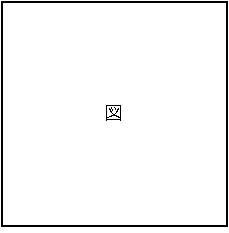
\includegraphics[height=40mm]{images/pdf/figure}
        \subcaption{Learning phase}
    \end{minipage}
    \begin{minipage}[c]{65mm} 
        \centering
        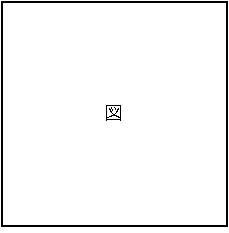
\includegraphics[height=40mm]{images/pdf/figure}
        \subcaption{Following phase}
    \end{minipage}
    \caption{Sequence of the experiment}
    \label{Fig:Sequence of the experiment}
  \end{figure}

\newpage
